% -*- Mode:TeX -*-
% LaTeX template for CinC papers                   v 1.1a 22 August 2010
%
% To use this template successfully, you must have downloaded and unpacked:
%       http://www.cinc.org/authors_kit/papers/latex.tar.gz
% or the same package in zip format:
%       http://www.cinc.org/authors_kit/papers/latex.zip
% See the README included in this package for instructions.
%
% If you have questions, comments or suggestions about this file, please
% send me a note!  George Moody (george@mit.edu)
%
\documentclass[twocolumn]{cinc}
\usepackage{graphicx}
\begin{document}
\bibliographystyle{cinc}

% Keep the title short enough to fit on a single line if possible.
% Don't end it with a full stop (period).  Don't use ALL CAPS.
\title{Heart Murmur Detection from Phonocardiogram Recordings: \\
George B.\ Mood PhysioNet Challenge 2022}

% Both authors and affiliations go in the \author{ ... } block.
% List initials and surnames of authors, no full stops (periods),
%  titles, or degrees.
% Don't use ALL CAPS, and don't use ``and'' before the name of the
%  last author.
% Leave an empty line between authors and affiliations.
% List affiliations, city, [state or province,] country only
%  (no street addresses or postcodes).
% If there are multiple affiliations, use superscript numerals to associate
%  each author with his or her affiliations, as in the example below.

\author {Enoch Guo
\ \\ % leave an empty line between authors and affiliation
  Stony Brook School, New York}

\maketitle
\begin{abstract}

We present a machine learning method for heart murmur detection from phonocardiogram (PCG) recordings. Our approach consists of three steps: (1)~Split recordings into 3-second waveforms; (2)~Transform one-dimensional waveforms into two-dimensional time-frequency heat maps using Mel-Frequency Cepstral Coefficients (MFCC); (3) Classify MFCC using deep convolutional neural networks (CNN). We also use denoising autoencoder classification to improve the basic CNN.

\end{abstract}

\section{Introduction}

The goal of the Challenge is to identify the presence, absence, or unclear cases of murmurs and the normal vs. abnormal clinical outcomes from heart sound recordings collected from multiple auscultation locations on the body using a digital stethoscope.

%\subsection{Dataset}

The Challenge data contain one or more heart sound recordings for 1568 patients as well as routine demographic information about the patients from whom the recordings were taken. The Challenge labels consist of two types:

\begin{enumerate}
\item Murmur-related labels indicate whether an expert annotator detected the presence or absence of a murmur in a patient from the recordings or whether the annotator was unsure about the presence or absence of a murmur.
\item Outcome-related labels indicate the normal or abnormal clinical outcome diagnosed by a medical expert.
\end{enumerate}

The Challenge data is organized into three distinct sets: training, validation, and test sets. The organizers have publicly released 60\% of the dataset as the training set of the 2022 Challenge, and have retained the remaining 40\% as a hidden data for validation and test purposes. 

Therefore, we are given the training set that contains 3163 recordings from 942 patients. The public training set contains heart sound recordings, routine demographic information, murmur-related labels (presence, absence, or unknown), outcome-related labels (normal or abnormal), annotations of the murmur characteristics (location, timing, shape, pitch, quality, and grade), and heart sound segmentations. The private validation and test sets only contain heart sound recordings and demographic information.


%\subsection{Challenge Scoring}
%
%The result for each patient consists of the class label as well as a probability or confidence score for each class per subject ID.
%
%\begin{verbatim}
%#1234
%Present, Unknown, Absent, Abnormal, Normal
%       1,      0,      0         1,      0
%    0.75,   0.15,    0.1       0.6,    0.4
%\end{verbatim}
%
%The two scoring metrics are defined in terms of the following confusion %matrices for murmurs and clinical outcomes.



\section{Split into 3-second waveforms}

The PCG recordings have different lengths, varying from 20608 to 258048 data points; with daterate being 4000 samples/sec, they vary from 5 seconds to about one minute.

PCG consists of cycles; each cycle consists of four states: S1, S2, systole and diastole. 
We split each recording into 3-second long overlapping segments, which is long enough to determine abnormality of heart sound.
Each split wave consists of 12000 data points.

\section{MFCC}

Mel-Frequency Cepstral Coefficients (MFCC) \cite{mfcc} has been widely used in speech recognition. We extract 4 frequency bands, because if we extracted more frequency bands, other frequency bands would be mostly empty. Thus each one-dimensional wave (12000 long) is transformed into a two-dimensional heat map, of size $(4, 201)$, using ${\tt win\_length}=100$ and ${\tt hop\_length}=60$. 

\section{Basic CNN}

We use three layers of convolution.
\begin{enumerate}
\item Encode:
\begin{enumerate}
\item Conv2d
\item BatchNorm2d
\item ReLU
\item Conv2d
\item BatchNorm2d
\item ReLU
\item Conv2d
\item BatchNorm2d
\item ReLU
\item Flatten
\end{enumerate}
\item Classify:
\begin{enumerate}
\item Dense
\item ReLU
\item Dense
\item Softmax
\end{enumerate}
\end{enumerate}

\section{Denoising Autoencoder Classification}

\begin{figure}[h]
\centering
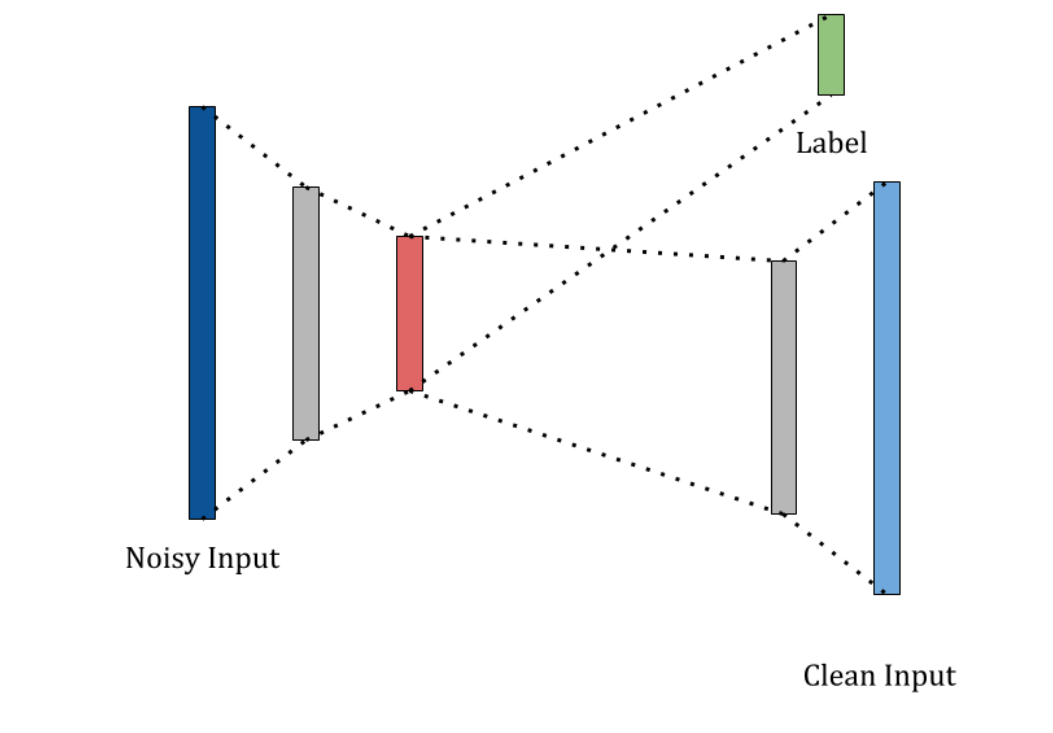
\includegraphics[width=7.9cm]{dac.png}
\caption{Denosing Autoencoder Classification Model}
\label{FIGURA1}
\end{figure}

\textbf{Training algorithm}: Let $X$ be input points (cyan), of size $(C,W,H)=(1, 4,201)$, and $Y$ be the classification labels (green).
\begin{enumerate}
\item Add noise: $X'={\it add\_noise}(X)$. $X'$ is blue. We have two methods to add noise: blackout and random. Blackout method chooses a small sample points (10\%) to zero out their values; Random method changes the values by randomly with $\mu=0$ and a small $\sigma$, say, 0.1.
\item Denoising autoencoder decode: Let $Z$ be the latent layer (red). We train $X'\to Z\to (Y, X)$, where $X'\to Z$ is encode; $Z\to Y$ is classify; and $Z\to X$ is decode (decode consists of the reversed steps of encode). In this step, the loss function for classify is zero. The model is called regularized after this step.
\item Classify from the regularized model: continue to train using cross entropy loss function for classify: $Z\to Y$.

\end{enumerate}

Each step in Decode is the inverse function of the 
corresponding Encode step, in reverse order.

\begin{enumerate}\addtocounter{enumi}{2}
\item Decode
\begin{enumerate}
\item Unflatten
\item ConvTranspose2d
\item BatchNorm2d
\item ReLU
\item ConvTranspose2d
\item BatchNorm2d
\item ReLU
\item ConvTranspose2d
\item Sigmoid
\end{enumerate}
\end{enumerate}


%All references should be included in the text in square brackets in their
%order of appearance, e.g., \cite{tag}, \cite{tag,ito}, or
%\cite{tag,ito,fardel,buncombe}. In the reference list, use the Vancouver
%style (see IEEE Transactions on Biomedical Engineering or Annals of
%Biomedical Engineering). The main goal is to be consistent in your
%formatting of references.



% \section*{Acknowledgments}  

\bibliography{refs}

\begin{thebibliography}{99}{ %\small
 
 \bibitem{mfcc} T. Ganchev, N. Fakotakis, G. Kokkinakis, ``Comparative Evaluation of Various MFCC Implementations on the Speaker Verification Task,'' 
 \emph{Proc. of the SPECOM-2005}, October 17-19, 2005. Patras, Greece. Vol. 1, pp.191-194.
 

      
}\end{thebibliography}


%\begin{correspondence}
%My Name\\
%My Full postal address\\
%My E-mail address
%\end{correspondence}

\end{document}

